\chapter{Modelo de iluminación}
\section{Introducción}
En este capítulo vamos a ver los principios de los modelos de iluminación, así como operadores importantes. Seguidamente presentaremos el modelo de iluminación Phong, que es y ha sido utilizado desde los años 70.\\\\Un modelo de iluminación es esencial para el diseño artístico de la escena, simular propiedades físicas como por ejemplo, reflejos, refracción, etc. Además, las sombras dan sensación de profundidad a una escena.\\\\
En este capítulo hablaremos de dos elementos importantes, luces y sombras. Aunque no lo parezca, todos ellos hacen uso de una propiedad fundamental de las superficies, el vector normal. Vamos a crear el algoritmo definidio en el apatartado \textit{Preliminares}.
\begin{lstlisting}
// Cálculo de la normal de la isosuperficie estimado por un rayo.
vec3 Normal(vec3 p){
     // f(x1,...,xn)
     float fxyz = escena_sdf(p);
     // f(x1,..,xi+h,xn)
     float fxhyz = escena_sdf(p + vec3(EPSILON, 0.0, 0.0));
     float fxyhz = escena_sdf(p + vec3(0.0, EPSILON, 0.0));
     float fxyzh = escena_sdf(p + vec3(0.0, 0.0, EPSILON));
     // Utilizamos la definicion de derivadas parciales para devolver el gradiente, que se trata de la normal de la isosuperficie, como hemos definido en los Preliminares.
     return vec3(
         (fxhyz - fxyz) / EPSILON,
         (fxyhz - fxyz) / EPSILON,
         (fxyzh - fxyz) / EPSILON
     );
}
\end{lstlisting}
\newpage
Vamos a ahora a presentar el \textit{producto escalar}, implementado de forma nativa en \textit{GLSL} con el nombre de "\textit{dot}", esencial para los modelos de iluminación.
\[\Vec{r} \cdot  \Vec{v} = r_xv_x + r_yv_y + r_zv_z = \vert r\vert\vert v\vert\cos(\alpha)\]
Si ambos son vectores directores, es decir, normalizados y en el origen, resulta \(\Vec{r} \cdot \Vec{v} = \cos(\alpha)\). El valor \(\alpha\) es el ángulo entre los dos vectores sobre el plano que forman, en caso de \(\mathbb{R}^2\), la componente \(z\) sería nula. La imagen del operador es el intervalo \([-1,1]\)\\Veamos alguna de las propiedades, si ambos vectores son perpendiculares, con \(\alpha=\pm\dfrac{\pi}{2}\), el \textit{producto escalar} será \(\Vec{r}\cdot\Vec{v}=\cos\left(\pm\dfrac{\pi}{2}\right)=0\). En el caso en el que sean son paralelos, \(\alpha=\{0,\pi\}\), el resultado será  \(\Vec{r}\cdot\Vec{v}=\cos(\{0, \pi\})=\pm 1\), según la dirección de ambos.\\\\ El lenguaje \textit{GLSL} presenta dos operaciones vectoriales que utilizaremos en modelo, estas son.
%https://es.m.wikipedia.org/wiki/Ley_de_Snell
\begin{table}[h]
    \begin{tabularx}{\textwidth}{l|X}
        \toprule
        Función & Definición\\
        \midrule
        \pbox{10cm}{
          reflect(\\
          \tab[1cm]vecN a,\\
          \tab[1cm]vecN n, \\
          )} & El vector \(\Vec{n}\) debe estar normalizado, este operador devuelve el vector \(\Vec{a}\) reflectado respecto de \(\Vec{n}\),
        \[\Vec{r}=\Vec{a} - 2(\Vec{n} \cdot \Vec{a})\Vec{n}\]
        \begin{minipage}{1.0\textwidth}
          \centering
          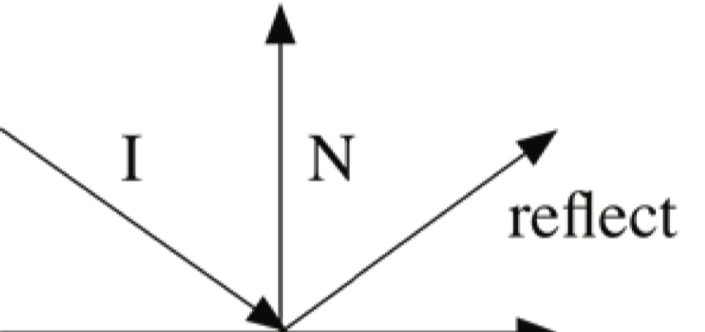
\includegraphics[width=.25\textwidth]{secciones/imagenes/reflect.jpeg}
        \end{minipage}
        \\
        \pbox{10cm}{
        refract(\\
          \tab[1cm]vecN a,\\
          \tab[1cm]vecN n, \\
          \tab[1cm]float k, \\
          )} & El vector \(\Vec{n}\) debe estar normalizado, este operador devuelve el vector \(\Vec{a}\) refractado respecto de \(\Vec{n}\), con \(k\) como factor de medio. Según la \textit{ley de refracción de Snell-Descartes}.
        \[\Vec{r}=k\left(\Vec{a} - \left(\left(\Vec{n} \cdot \Vec{a}\right)+\sqrt{\dfrac{1}{k^2}-(\Vec{a}\cdot\Vec{n})^2}\right)\Vec{n}\right)\]
        \begin{minipage}{1.0\textwidth}
          \centering
          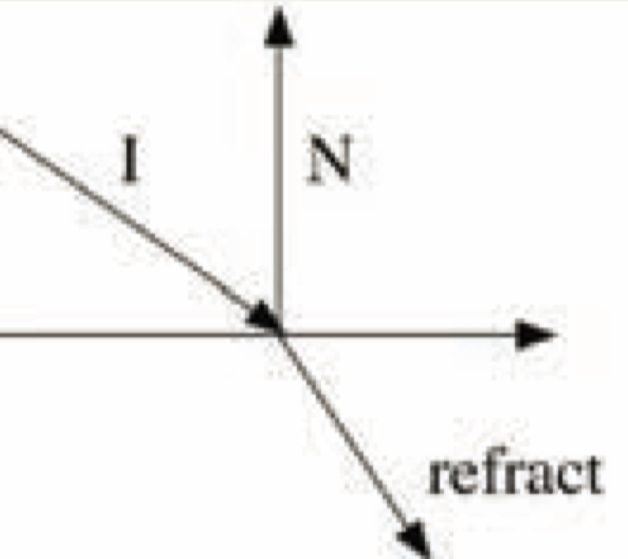
\includegraphics[width=.3\textwidth]{secciones/imagenes/refract.jpeg}
        \end{minipage}\\
        \bottomrule
    \end{tabularx}
\end{table}
\newpage
\section{Luz e Intensidad}
En este apartado veremos la definición de \textit{Intensidad lumínica}, así como dos tipos de luces existentes, luz direccional y radial.\\\\
 Definimos la \textit{intensidad lumínica} en un punto como un factor multiplicativo al material asignado al punto de la \textit{isosuperficie}, representa cómo de iluminado está. Como es un factor multiplicativo, el valor de \(0.0\), representa la intensidad nula u oscuridad. Mientras que el valor \(1.0\) representa el valor más iluminado.\\\\ 
El operador \textit{producto escalar} nos debería dar una breve intuición del papel importante que juega en el cálculo de la intensidad. Como esta no puede ser negativa, definimos el operador producto escalar positivo y normalizado "\(\cdot_{[0,1]}\)".
\[\cdot_{[0,1]}:\mathbb{R}^2\times\mathbb{R}^2\longrightarrow[0,1] : \Vec{a}\cdot_{[0,1]}\Vec{b}=\max\left(\dfrac{\Vec{a}\cdot \Vec{b}}{\vert\vert\Vec{a}\vert\vert\vert\vert \Vec{b}\vert\vert}, 0\right)\]
Vamos a utilizar el "\textit{Modelo de Iluminación de Phong}", presentado en 1973 por \textit{Tuong Phong} como un modelo de iluminación empírico. Para ello, vamos a ver como el modelo se descompone en tres etapas. La primera, el cálculo de la \textbf{Intensidad Ambiente}, que se trata de un valor \(I_a \in [0,1]\) que indica cuanto de iluminada está la isosuperficie, de manera inicial o si no hubieran luces. 
\begin{figure}[H]
  \centering
  \captionsetup{justification=centering}%,margin=2cm
  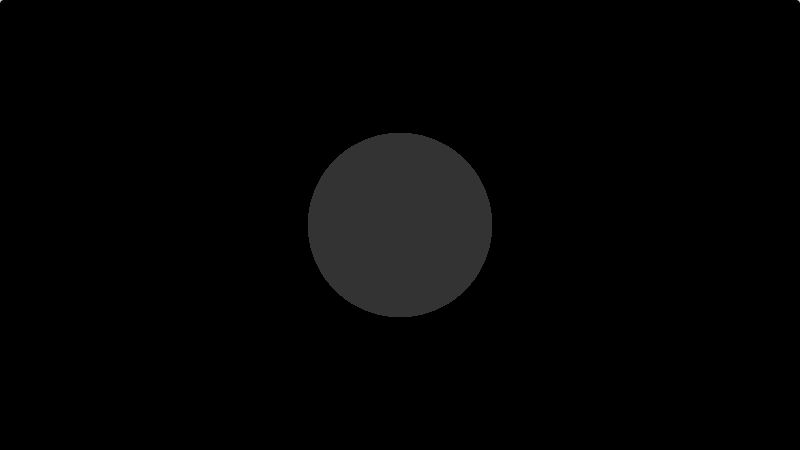
\includegraphics[width=0.8\textwidth]{secciones/imagenes/lightmodel/ambiental.png}\label{fig:ambient}
  \caption{Intensidad Ambiental sobre la esfera.}
\end{figure}
Por otro lado, la \textbf{Intensidad Especular}, que es aportada de manera colectiva sobre el punto aproximado \(\Vec{p}\) de la \textit{isosuperficie}, para cada una de las luces de la escena \(\Vec{l_i}\in L\), donde \(\Vec{l_i}\) representa la posición de la luz, se comprueba como incide la luz sobre la superficie, con respecto de su normal. 
\[I_d = \sum_{\Vec{l_i}\in L} \Vec{n}\cdot_{[0, 1]}(\Vec{l_i}-\Vec{p})\]
Donde \(\Vec{n}\) es la normal de la \textit{isosuperficie} en el punto \(\Vec{p}\). Es fácil observar que, la intensidad debería ser máxima cuando los rayos inciden en de manera paralela en sentido contrario al vector normal y nulo en caso de que sean perpendiculares u opuestos.
\begin{figure}[H]
  \centering
  \captionsetup{justification=centering}%,margin=2cm
  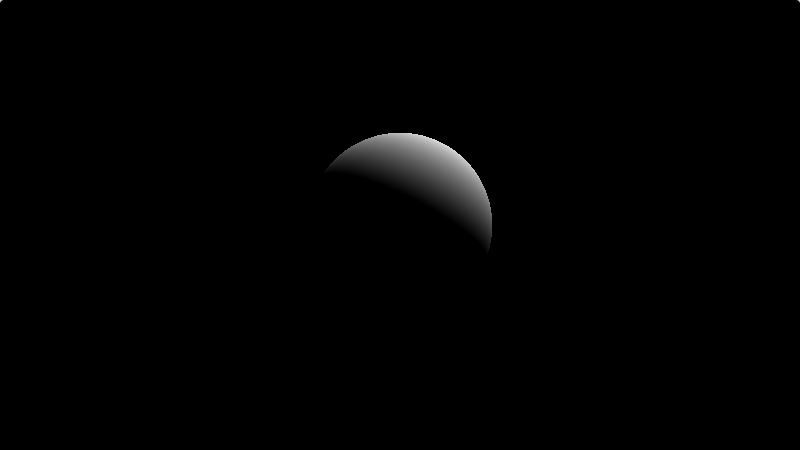
\includegraphics[width=0.8\textwidth]{secciones/imagenes/lightmodel/difusa.png}\label{fig:difusse}
  \caption{Intensidad Difusa sobre la esfera.}
\end{figure}
Veamos finalmente la \textbf{Intensidad Especular}, esta intensidad indica como incide la luz reflectada  por la \textit{isosuperficie} en el la dirección del ojo.\\
Definimos el operador de reflexión "\(\veebar\)"\footnote{La demostración la podemos encontrar en...}, de un vector \(\Vec{a}\) sobre un vector director \(\Vec{n}\).
\[\Vec{a}\veebar\Vec{n}=\Vec{a} - 2(\Vec{n} \cdot \Vec{a})\Vec{n}\]
La ecuación final de la "\textit{Intensidad Especular}" para todas las luces de la escena es,
\[I_e = \sum_{\Vec{l_i}\in L} \Vec{ojo}\cdot_{[0, 1]}\left(\left(\Vec{l_i}-\Vec{p}\right) \veebar \Vec{n}\right)\]
Algunos autores aportan una leve modificación de esta ecuación, aplicando un \textit{homomorfismo} polinómico con grado exponencial.
\[h_k:[0,1]\longrightarrow[0,1] , h_k(x)=x^{2^k}\]
\[I_d = \sum_{\Vec{l_i}\in L} h_k\left(\Vec{ojo}\cdot_{[0, 1]}\left(\left(\Vec{l_i}-\Vec{p}\right) \veebar \Vec{n}\right)\right)\]
Donde \(k\in\mathbb{R}^{+}\) y este tiene efecto sobre el radio de rayos reflejados.
\begin{figure}[H]
  \centering
  \captionsetup{justification=centering}%,margin=2cm
  \subfloat[Intensidad especular con \(h_0\)]{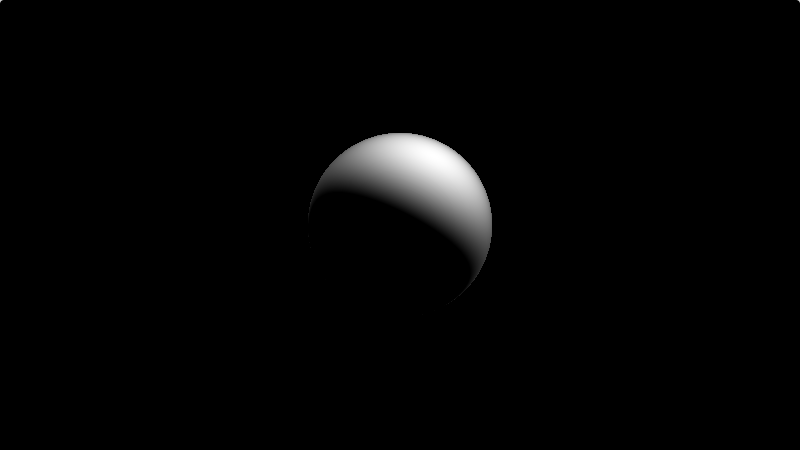
\includegraphics[width=0.33\textwidth]{secciones/imagenes/lightmodel/especular-0.png}\label{fig:specular-0}}
  \subfloat[Intensidad especular con \(h_1\)]{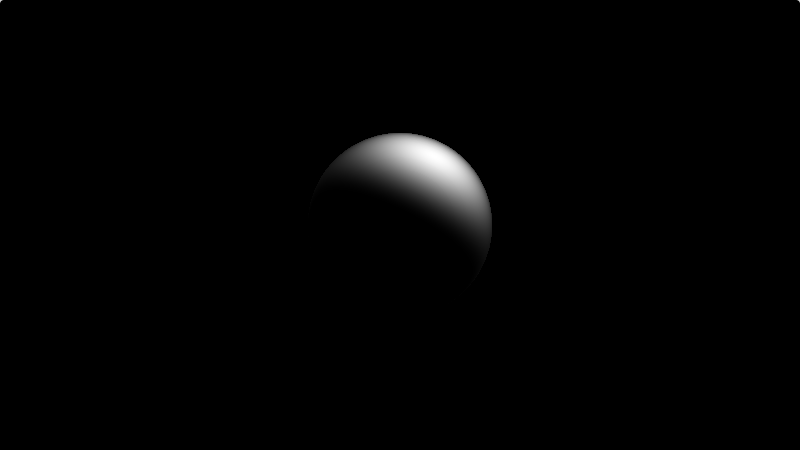
\includegraphics[width=0.33\textwidth]{secciones/imagenes/lightmodel/especular-1.png}\label{fig:specular-1}}
  \subfloat[Intensidad especular con \(h_3\)]{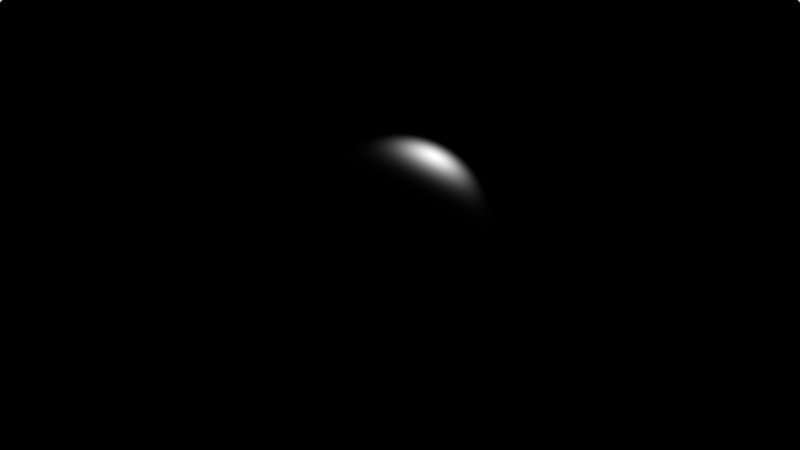
\includegraphics[width=0.33\textwidth]{secciones/imagenes/lightmodel/especular-2.png}\label{fig:specular-2}}
  \caption{Intensidad Difusa con distintos homomorfismos}
\end{figure}
El modelo final, definido por la \textit{Intesidad del modelo de Phong} se calcula como la suma de las intensidades expuestas anteriormente.
\[I_{Phong}=I_a+\sum_{\Vec{l_i}\in L} \mathrlap{\underbrace{\phantom{\Vec{n}\cdot_{[0, 1]}(\Vec{l_i}-\Vec{p})}}_{\text{Intensidad Difusa}}}\Vec{n}\cdot_{[0, 1]}(\Vec{l_i}-\Vec{p}) + \mathrlap{\underbrace{\phantom{h_k\left(\Vec{ojo}\cdot_{[0, 1]}\left(\left(\Vec{l_i}-\Vec{p}\right) \veebar \Vec{n}\right)\right)}}_{\text{Intensidad Especular}}}h_k\left(\Vec{ojo}\cdot_{[0, 1]}\left(\left(\Vec{l_i}-\Vec{p}\right) \veebar \Vec{n}\right)\right)\]
Como hemos dicho antes, este es un factor, multiplicativo, en particular, multiplica al valor del material o en este caso, el color \textit{rgba} devuelto que era, el blanco.
\begin{figure}[H]
  \centering
  \captionsetup{justification=centering}%,margin=2cm
  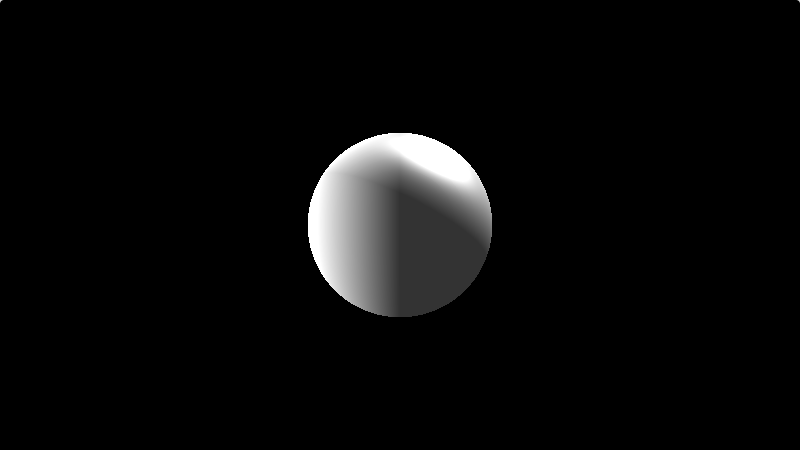
\includegraphics[width=0.8\textwidth]{secciones/imagenes/lightmodel/phong.png}\label{fig:phong}
  \caption{Intensidad Phong sobre la esfera con \(h_3\).}
\end{figure}
En algunas implementaciones, se utiliza para cada luz, un factor de atenuación que depende de la distancia de la superficie a la luz, esta función converge a cero en el infinito. En particular, OpenGL\footnote{A partir de la version X.X empezó...} utiliza la siguiente función:
\[p(x)=\dfrac{1}{ax^2+bx+c}\]
donde \(a,b,c \in \mathbb{R}^{+}_{0}\) son factores que dan una riqueza artística al modelo de iluminación, así como el \textit{homomorfismo} utilizado en la \textit{Intensidad Especular}.\\\\En luces direccionales, el punto se considera estar en el infinito, sustituyéndose \(\Vec{l_i}-\Vec{p}\) por el vector director de la luz \(\Vec{d_i}\). En caso de utilizar una función de atenuación, el valor que tomaría  será cero, por lo que la \textit{Intensidad Especular} quedaría anulada. Además, para la \textit{Intensidad Difusa}, utilizaremos el vector director de la luz direccional en vez de la diferencia del punto aproximado \(\Vec{p}\) y la posición de la luz \(\Vec{l_i}\).
\newpage
Veamos un ejemplo práctico en código.
\begin{lstlisting}
// Homomorfismo
float h3(float h){return pow(h,pow(2.,3.));}
// Definimos el operador producto escalar normalizado positivo.
float dot01(vec3 a, vec3 b){ 
    return max(dot(a,b)/(normalize(a)*normalize(b)), 0.0);
}
// Modelo de iluminación Phong
float ModeloIluminacion(vec3 direccion, vec3 p){
    // Calculamos la normal del punto.
    vec3 normal = Normal(p);
    // Ayuda al marcher a escapar de la isosuperficie
    p = p + normal * 0.1;
    // Modelo
    float intensidad = 0.0;
    // Intensidad Ambiente Global
    intensidad += 0.2;
    // Intensidad de cada Luz
    // Luz 1.
    vec3 posicion_luz_1 = vec3(2., 4., 1.);
    vec3 d_luz_1 = posicion_luz_1 - p;
    float dst_luz_1 = length(d_luz_1);
    // Intensidad Difusa
    intensidad += dot01(d_luz_1, normal);
    // Intensidad Especular, en caso de ser una luz direccional, podemos ignorar esta componente ya que la posición es considerada estar en el infinito y por ello, f_difusa = 0
    vec3 r_luz_1 = reflect(d_luz_1, normal);
    intensidad += f_difusa(dst_luz_1) * h3(dot01(r_luz_1, direccion));
    // ... Utilizamos el mismo esquema para las demás luces.
    // Devolvemos la intensidad en el rango [0, 1].
    return clamp(intensidad, 0.0, 1.0);
}
\end{lstlisting}
\newpage
\section{Sombras}
Vamos a ver la técnica más sencilla para calcular las sombras, pero es importante mencionar que hablaremos únicamente de la \textit{umbra} de una la sombra. La \textit{umbra} sucede cuando la fuente de luz es ocluida completamente por una superficie. Haciendo que la luz no actue sobre la intensidad del punto.\\\\Una vez aproximado un punto \(p\) de la \textit{isosuperficie}, diremos que está en \textit{umbra}, si es ocluido por un objeto en dirección a la luz, o lo que es lo mismo, podemos utilizar el marcher desde \(\Vec{p}\) en dirección a la luz \(\Vec{l_i}\), cuyo plano trasero contiene a \(\Vec{l_i}\). Si este traza otro punto \(\Vec{q}\) en esa dirección, este estará en \textit{umbra}.\\\\
Vamos a realizar una pequeña modificación sobre el vector \(\Vec{p}\) que ayudará a agilizar el \textit{Marcher}, ya que las primeras iteraciones de este, intentará "escapar" de la isosuperficie, para ello, vamos a empujarlo de la superficie, utilizando la normal.
\[\Vec{p'}=\Vec{p} + \Vec{n} \cdot k\]
Donde \(k\in\mathbb{R}^{+}_{0}\) y funciona como un factor de empuje de la superficie, se trata de un valor empírico que ayuda al marcher a salir de la isosuperficie, ya que en las primeras iteraciones, el radio de las esferas está muy próximo a \(0,0\). \\\\
% Imagen Desplazamiento 
Se ha realizado además una leve modificación del marcher, ahora este aceptará un tercer argumento, que indica la distancia del plano trasero, que anteriormente estaba fijado por el plano trasero \textit{MAXIMO}. Esto nos será útil para parar el marcher cuando hemos trazado la distancia la distancia a la luz.\\\\
Vamos a crear un modelo de iluminación con \textbf{dos} luces, una radial y otra direccional. Además, utilizaremos un plano en donde proyectar la sombra. La luz direccional es perpendicular al plano.
\begin{figure}[H]
  \centering
  \captionsetup{justification=centering}%,margin=2cm
  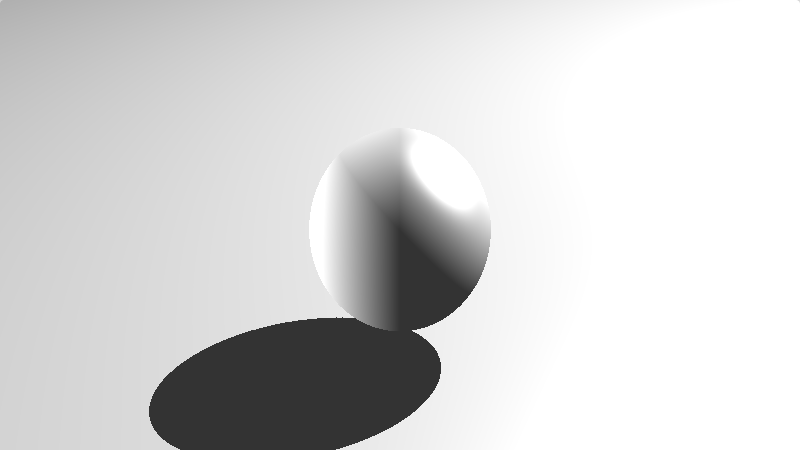
\includegraphics[width=0.8\textwidth]{secciones/imagenes/lightmodel/sombra_dura.png}\label{fig:shadow}
  \caption{Modelo de iluminación y sombras sobre la escena definida.}
\end{figure}
\newpage
\begin{lstlisting}
// Se ha añadido un tercer argumento.
float SphereMarching(in vec3 ojo, in vec3 direccion, float distancia_plano){
    float distancia = 0.0;
    for(int i = 0; i < PASOS; ++i){
        vec3 rayo = ojo + direccion * distancia;
        float radio = escena_sdf(rayo);
        if(radio < EPSILON){
            return distancia;
        }
        distancia += radio;
        // Ahora depende del tercer argumento
        if(distancia > distancia_plano)break;
    }
    return distancia_plano;
}
// Phong + Sombras duras
float ModeloIluminacion(vec3 direccion, vec3 p){
    // Calculamos la normal del punto.
    vec3 normal = Normal(p);
    // Ayuda al marcher a escapar de la isosuperficie
    p = p + normal * 0.1;
    // Modelo
    float intensidad = 0.0;
    // Intensidad Ambiente Global
    intensidad += 0.2;
    // Luz 1.
    vec3 posicion_luz_1 = vec3(2., 4., 1.);
    vec3 d_luz_1 = posicion_luz_1 - p;
    vec3 dir_luz_1 = normalize(d_luz_1);
    float dst_luz_1 = length(d_luz_1);
    // En el caso de que se trate de una luz direccional, utilizaremos el plano MAXIMO, utilizado antes.
    if(SphereMarching(pd, dir_luz_1, dst_luz_1) >= dst_luz_1){
        // Intensidad Difusa
        intensidad += dot01(d_luz_1, normal);
        // Intensidad Especular (Si no es direccional)
        vec3 r_luz_1 = reflect(d_luz_1, normal);
        intensidad += f_difusa(dst_luz_1) * h3(dot01(r_luz_1, direccion));
    }
    // ... Repetimos el esquema anterior.
    return clamp(intensidad, 0.0, 1.0);
}
\end{lstlisting}
%https://www.shadertoy.com/view/wtfBW8
\newpage
